\documentclass[10pt]{article}


\usepackage{amsmath}
\usepackage{amssymb}
\usepackage{array}
\usepackage[english]{babel}
\usepackage{blindtext}
\usepackage{booktabs}
\usepackage{ctable}
\usepackage{enumitem}
\usepackage{fancyhdr}
\usepackage{float}
\usepackage[a4paper, margin=0.5in]{geometry}
\usepackage[utf8x]{inputenc}
\usepackage{graphicx}
\usepackage{mathrsfs}
\usepackage{placeins}
\usepackage{rotating}
\usepackage{ragged2e}
\usepackage{relsize}
\usepackage{tabularx}
\usepackage{url}
\usepackage{xcolor,colortbl}


% Quotes
\newcommand{\qn}[1]{``#1''}


\title{\textbf{An Alpha-Beta Pruning Algorithm for the Ultimate Tic-Tac-Toe Game}}
\author{Thiago V. de A. Silva\\2017719891}
\date{\today}
\begin{document}

\maketitle

\section{Introduction}

Tic-Tac-Toe is a classic 2-player game. Given a 3x3 board, the game takes place in turns, in each turn a player has to choose a blank square in the grid and put his mark on it, whoever gets three marks in a row wins. This game is extensively used as example in artificial intelligence and game theory courses. In this report, we define the player's 1 mark as X and player's 2 as O.

\begin{figure}[h]
\centering
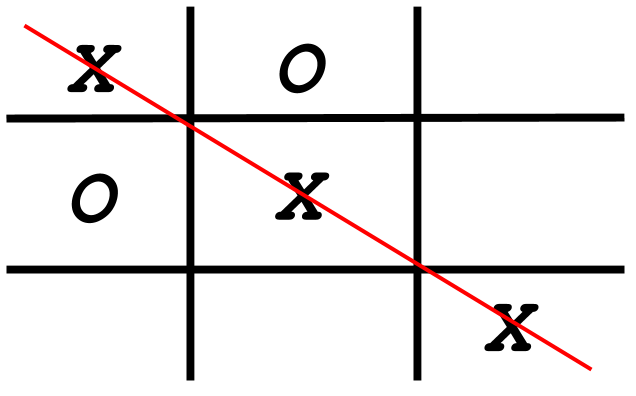
\includegraphics[scale=0.2]{img/tic-tac-toe.png}
\caption{Example of tic-tac-toe game; player 1 won!}
\end{figure}

 There are several variations of the game: 3D tic-tac-toe, Wild tic-tac-toe, Ultimate tic-tac-toe... \cite{3dtictactoe,wildtictactoe,ultimatetictactoe}. On this project, we decided to work with the ultimate version of the game. This variation is interesting because it's simple, there is no clear winning strategies, unlike the classic version, and the number of states is exponentially high.\\
 
In this work, we've implemented an alpha-beta pruning algorithm for the ultimate tic-tac-toe, and tested it considering two distinct payoff tables, and we've done a sanity test running our proposed solutions against a player that selects random positions.

\section{Game Rules}
The Ultimate tic-tac-toe is a 2-player game, just like the classic version. Given a 3x3 board, for each square there is a classic tic-tac-toe board, see the figure below for better understanding:

\begin{figure}[h]
\centering
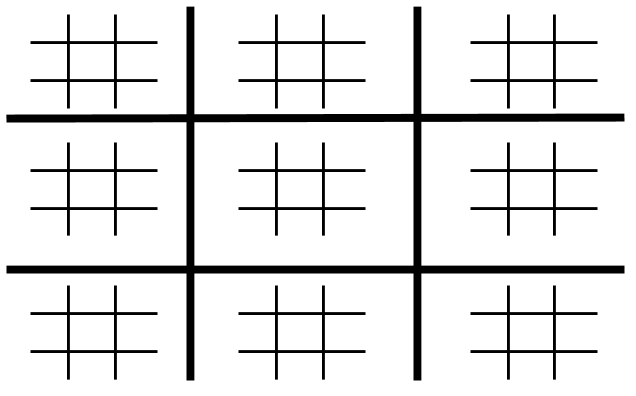
\includegraphics[scale=0.3]{img/ultimate.png}
\caption{Example of the Ultimate tic-tac-toe game}
\end{figure}

% inner and outter

The game takes place in turns: The first player starts, he chooses any inner board and put his mark in a blank square on position (i, j) of the inner game, then player 2 must play at the (i, j) board. For example: Suppose player 1 chooses the (1, 0) inner game, and marked at position (1, 2); then, player 2 must play the (1, 2) inner game next, in the figure below she played at the position (0, 0) of the (1, 2) inner board, then player 1 must play the (0, 0) inner board, and this game goes on...\\

Each play is defined by four coordinates $(x, y, i, j)$, in which $(x, y)$ indicates the outer position and $(i, j)$ indicates the inner position. Given that the first player played at $(x_1, y_1, i_1, j_1)$, for instance, then player 2 must play at $(i_1, j_1, i_2, j_2)$ next. See the example below:

\begin{figure}[h]
\centering
\begin{minipage}{.33\textwidth}
  \centering
  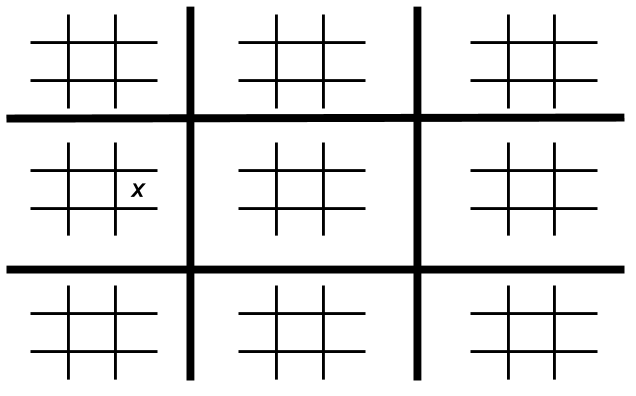
\includegraphics[width=.9\linewidth]{img/ultimate1.png}
  \caption{First turn}
\end{minipage}%
\begin{minipage}{.33\textwidth}
  \centering
  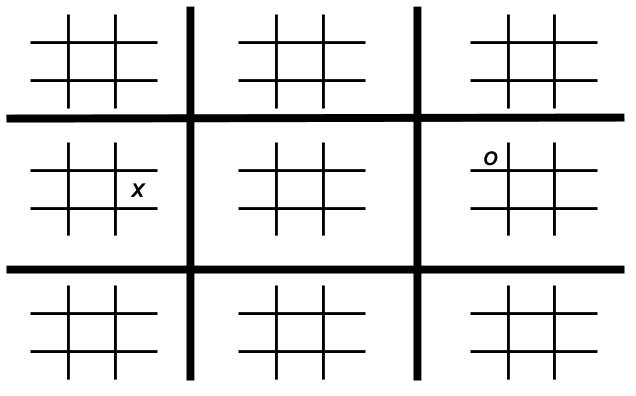
\includegraphics[width=.9\linewidth]{img/ultimate2.png}
  \caption{Second turn}
\end{minipage}
\begin{minipage}{.33\textwidth}
  \centering
  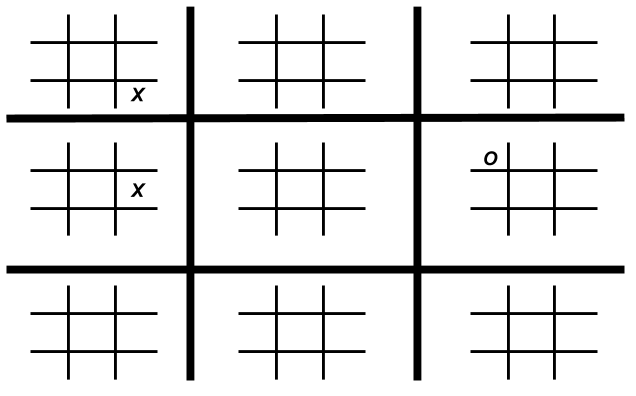
\includegraphics[width=.9\linewidth]{img/ultimate3.png}
  \caption{Third turn}
\end{minipage}
\end{figure}

In case player 2 is sent to an inner board that is already full or any player had already won that inner game, then she can play wherever she wants in the entire game.\\
If a player wins an inner game, than he gets to put a big mark on the outer position of the game he'd won. e.g.:

\begin{figure}[h]
\centering
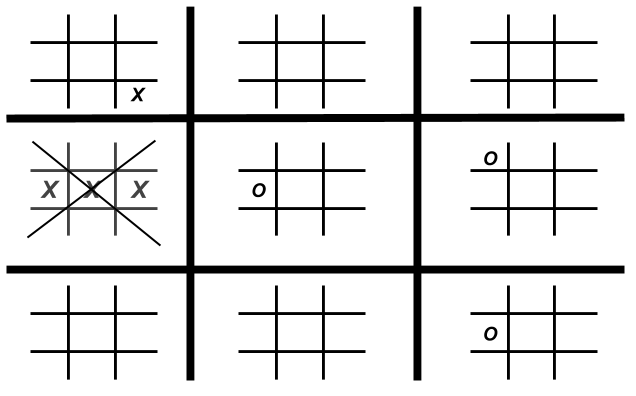
\includegraphics[scale=0.3]{img/ultimate4.png}
\end{figure}

Whoever gets three marks in a row on the outer board, wins the game.\\

\section{Payoff Tables}
We've designed two distinct payoff tables for this game, their assembling was done in order to resemble known strategies of the classic tic-tac-toe game.\\

Each strategy is defined in two parts, outer payoffs and inner payoffs. The outer payoffs corresponds to plays in which players conquers a big mark. The inner payoffs corresponds to events in which just inner boards are altered. For every strategy, if the player gets to a state in which it has won the game, then he gets a payoff $p = +\infty$, and a state in which it has lost has payoff $p = -\infty$.\\

The inner payoffs are the same for all strategies: Every time a play doesn't affect the outer board, the inner payoff is set to $p_i = m_c - m_{opp}$, the number of marks of the current player present at the inner game minus the number of marks of the opponent; $p_i = 0$ otherwise. 

\subsection{Conquer Center First}
Hereafter abbreviated to CCeF, this payoff table tries to reflect the fact that, considering the classic board, there are more winning states in which the center square is used. There are $4$ winning states in which the center square is used, both diagonals in a row, the column and the row. For the corners, there are $3$ winning states for each one of them, the diagonal, the row and the column each one belongs to. And for the rest of the squares of the board, there are just two winning states for each one of them, the row and the column it belongs to. Hence, comes the payoff table:

\begin{figure}[H]
\centering
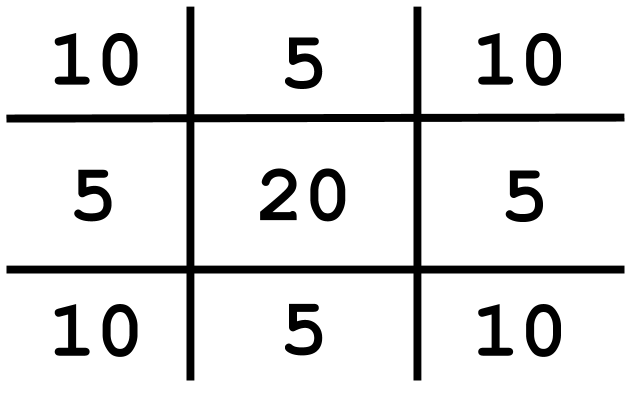
\includegraphics[scale=0.2]{img/ptable1.png}
\caption{CCeF's payoff table}
\end{figure}

So, if player 1 puts a big mark on the center, for instance, he gets $20$ points, but if player 2 puts a big mark on the center, then player 1 gets $-20$ points.

\subsection{Conquer Corners First}
Hereafter abbreviated to CCoF, this payoff table tries to mimic situations like this:

\begin{figure}[H]
\centering
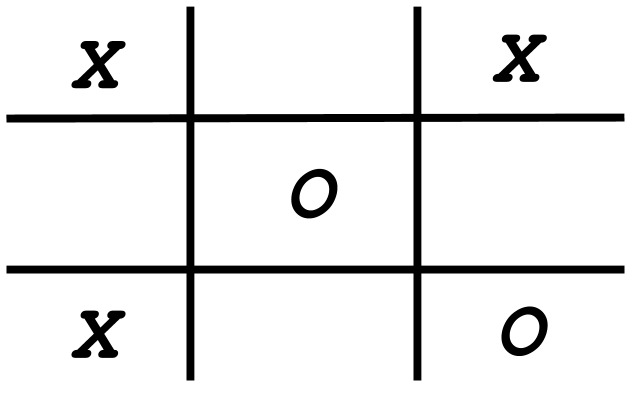
\includegraphics[scale=0.2]{img/situation1.png}
\end{figure}

Given that player 1 started, at this state, he has a sure win. In this strategy, the corners are more valuable, because we need to form a triangle in a any way to reach a unbeatable state. So, following this strategy, the corners has bigger payoffs than the other squares. Hence, comes the payoff table:

\begin{figure}[H]
\centering
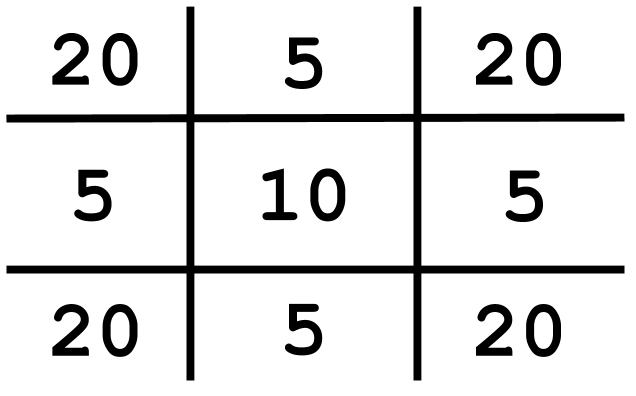
\includegraphics[scale=0.2]{img/ptable2.png}
\caption{CCeF's payoff table}
\end{figure}


\section{AI}

We've implemented two kinds of players in this work. One that always plays randomly and one that plays by looking into forward states of the game.

\subsection{Random}
This kind of player always chooses random places to play. We've measured some numbers that can help understand the game itself, and maybe the results presented afterwards.\\

We've put two Random AI's to play against each other $10^3$ times. Reminding that player 1 always starts.

\begin{figure}[H]
\centering
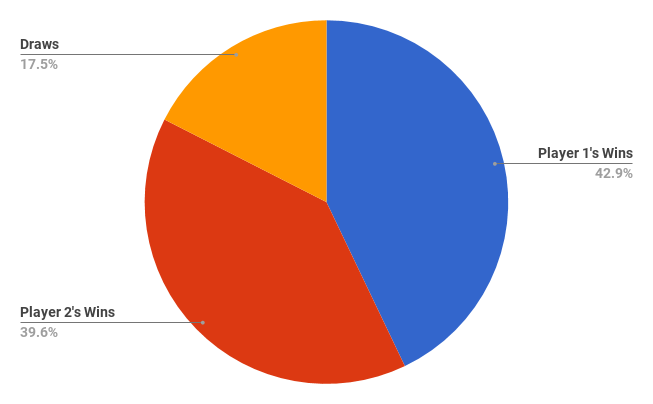
\includegraphics[scale=0.4]{img/random-chart.png}
\end{figure}

Analyzing the numbers, we can see that player 1 had a little advantage by starting the game.\\
We've also measured the number of moves done from the start of the game until the end.

\begin{figure}[H]
\centering
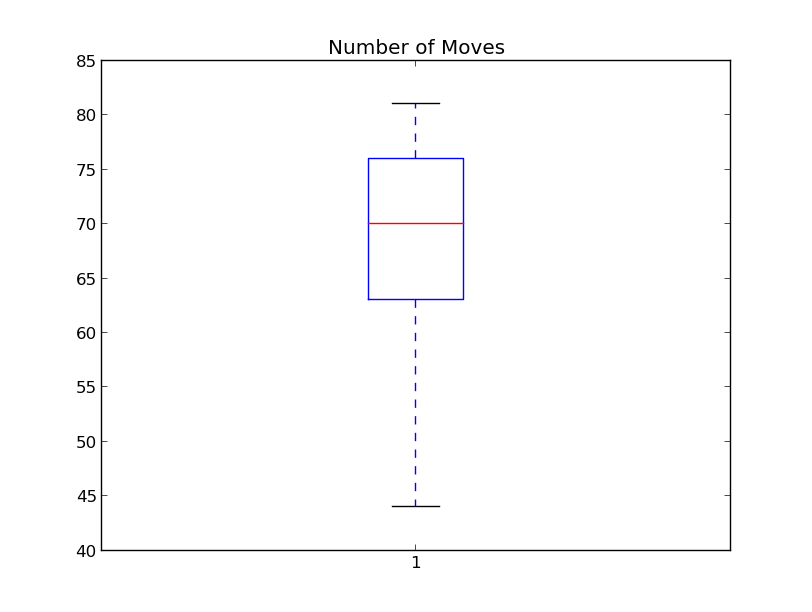
\includegraphics[scale=0.35]{img/n_moves_random.png}
\end{figure}

We can see that most of the games lasted from 63 to 76 moves.


\subsection{Alpha-Beta Pruning}
This is the second of kind of player we've implemented at this work. It can use either the CCeF or the CCoF strategies.\\
The player, basically, analyzes the tree of possibilities; and we implemented the alpha-beta pruning to improve the efficiency of the solution. At the beginning of the game, the player explores at most 4 levels of the tree of possibilities. By the ending of the game, we expand the branching to the sixth level of the tree, since by the ending of the game, the branching factor of each node of the tree gets narrowed to few moves.

\section{Experiments}

We've put some AI's to play with each other, and here we present the results we got.\\
The experiments performed were done as follows: For each setting presented here, we run 500 experiments. For each experiment a random starting point is choosen, and then we run 2 games, on the first player 1 starts playing, on the second player 2 starts playing. This is done to avoid getting biased results, due to the fact that the starting player has a little advantage over the other.

\subsection{Technical Details}
Every method or algorithm described in this report was implemented in python. The whole implementation can be found in \url{https://github.com/thiagovas/Ultimate-Tic-Tac-Toe}.\\
All experiments were executed in a Intel$^\copyright$ Core {\tiny\texttrademark} 2 Duo CPU E7500 with 2 cores of 2.93GHz, and with 4Gb of RAM.

\subsection{Sanity Test}
We put a CCeF and a CCoF player against a random player. This is just a sanity check to see how these players behave facing a random one.

\begin{figure}[h]
\centering
\begin{minipage}{.49\textwidth}
  \centering
  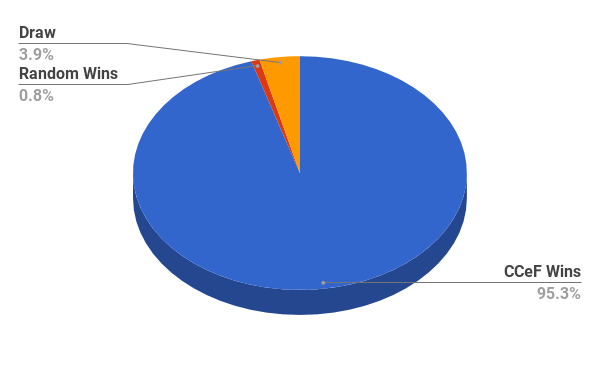
\includegraphics[width=.9\linewidth]{img/ccef-random.png}
  \caption{CCeF againt Random}
\end{minipage}%
\begin{minipage}{.49\textwidth}
  \centering
  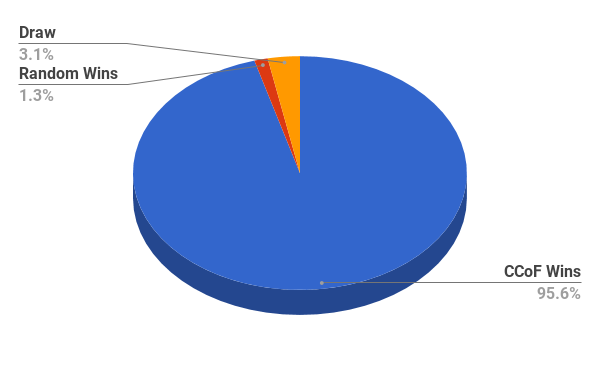
\includegraphics[width=.9\linewidth]{img/ccof-random.png}
  \caption{CCoF against Random}
\end{minipage}
\end{figure}

By looking at the results, we can see that the CCeF and CCoF are, by far, better than the random. We can notice as well that the CCeF was a little bit better than the CCoF, given that CCeF lost less.

\newpage
\subsection{CCeF vs CCoF}
We've also put CCeF to play against CCoF. The results can be seen below:

\begin{figure}[H]
\centering
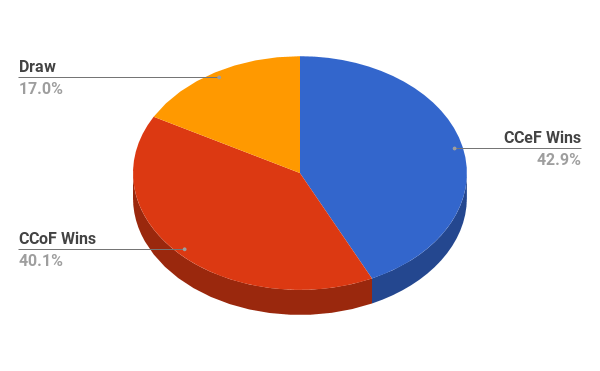
\includegraphics[scale=0.5]{img/ccef-ccof.png}
\end{figure}

By analyzing the results, we can see that the performance of CCeF and CCoF are very close, and CCeF outperformed CCoF by little ($2.8\%$). And the number of draws were significantly higher than the previous settings.


\section{Future Work}
As future work, there are four items that can be worked upon to improve the efficiency and quality of the AI for the game.\\
(1) There is another algorithm that can be applied to play the Ultimate Tic-Tac-Toe, the Monte Carlo Tree Search (MCTS). The MCTS has been used for other games, and it may work well for this game.\\
(2) Create more payoff tables. These payoff tables were created with a set of strategies in mind, they may not be the best payoff tables, and there is room for improvement in this point.\\
(3) Given that we've implemented all methods and algorithms in Python, we can consider using cython, or any optimizer. Because then the players could explore more possibilities at a time.\\
(4) Whitney et al. showed in \cite{george2016group} what are the equivalent classes of boards there are for the Ultimate Tic-Tac-Toe. Their work could serve to improve the efficiency of the AI's by improving the pruning of the tree of possibilities.
(5) Publish the AI's with an interface, so people could play against them.

\section{Conclusion}
In this work, we've implemented two strategies to play the Ultimate Tic-Tac-Toe game. We analyzed their behavior when playing with each other. And analyzed some characteristics of the game, as the average number of plays of the game, and as the player 1 having a little advantage starting the game.


\bibliography{report}{}
\bibliographystyle{plain}

\end{document}